\documentclass[12pt,twoside]{article}
\usepackage[russian,english]{babel}
\usepackage[utf8]{inputenc}
\usepackage{abstract}
\usepackage{amsmath,amssymb,mathrsfs,mathtext,amsthm}
\usepackage{a4wide}
\usepackage[T2A]{fontenc}
\usepackage{subfig}
\usepackage{url}
\usepackage[usenames]{color}
\usepackage{colortbl}

\newcommand{\hdir}{.}
\usepackage{hyperref}       % clickable links
\usepackage{lineno}
\usepackage{graphicx,multicol}
\usepackage{epstopdf}
\usepackage{cite}
\usepackage{amsmath,amssymb,mathrsfs,mathtext}
\usepackage{tikz}
\usetikzlibrary{shapes,arrows,shadows}

\newtheorem{theorem}{Theorem}
\newtheorem{proposition}{Proposition}

\theoremstyle{definition}
\newtheorem{definition}{Definition}

\usepackage{algorithm}
\usepackage[noend]{algcompatible}

\usepackage{multirow}

\usepackage{caption}

%\renewcommand{\baselinestretch}{1.4}


\newcommand{\bx}{\mathbf{x}}
\newcommand{\by}{\mathbf{y}}
\newcommand{\bw}{\mathbf{w}}
\newcommand{\ba}{\mathbf{a}}
\newcommand{\bb}{\mathbf{b}}
\newcommand{\bY}{\mathbf{Y}}
\newcommand{\bX}{\mathbf{X}}
\newcommand{\bu}{\mathbf{u}}
\newcommand{\bt}{\mathbf{t}}
\newcommand{\bp}{\mathbf{p}}
\newcommand{\bq}{\mathbf{q}}
\newcommand{\bc}{\mathbf{c}}
\newcommand{\bP}{\mathbf{P}}
\newcommand{\bT}{\mathbf{T}}
\newcommand{\bB}{\mathbf{B}}
\newcommand{\bQ}{\mathbf{Q}}
\newcommand{\bC}{\mathbf{C}}
\newcommand{\bE}{\mathbf{E}}
\newcommand{\bF}{\mathbf{F}}
\newcommand{\bU}{\mathbf{U}}
\newcommand{\bW}{\mathbf{W}}
\newcommand{\bbR}{\mathbb{R}}
\newcommand{\cA}{\mathcal{A}}
\newcommand{\T}{\mathsf{T}}
\newcommand{\bchi}{\boldsymbol{\chi}}
\newcommand{\bnu}{\boldsymbol{\nu}}
\newcommand{\bmu}{\boldsymbol{\mu}}
\newcommand{\btheta}{\boldsymbol{\theta}}
\newcommand{\bTheta}{\boldsymbol{\Theta}}
\newcommand{\bOne}{\boldsymbol{1}}
\newcommand{\bZero}{\boldsymbol{0}}
\newcommand{\argmin}{\mathop{\arg \min}\limits}
\newcommand{\argmax}{\mathop{\arg \max}\limits}

\newcommand\undermat[2]{%
	\makebox[0pt][l]{$\smash{\underbrace{\phantom{%
					\begin{matrix}#2\end{matrix}}}_{\text{$#1$}}}$}#2}


\begin{document}
	
	\linenumbers
	
	\title
{Multicorrelation}
\date{}
\maketitle
\begin{center}
	R.\,V.~Isachenko,
	V.\,V.~Strijov
\end{center}
\textbf{Abstract:} 
TBA

\bigskip
\textbf{Keywords}: TBA

\section{Feature categorization}
Feature selection algorithms eliminate features which are not relevant to the target variable.
To determine whether the feature is relevant the t-test could be applied for the correlation coefficient
\[
	r = \text{corr} (\bchi, \bnu), \quad t = \frac{r \sqrt{m - 2}}{1 - r^2} \sim \text{St} (m - 2);
\]
\begin{align*}
&H_0: r = 0; \\
&H_1: r \neq 0.
\end{align*}
If features are relevant, but correlated, feature selection methods pick the subset of them to reduce the multicollinearity and redundancy.
The goal is to find relevant, non-correlated features.
However, in this case the correlations between targets in matrix~$\bY$ are crucial.
To measure the dependence of each feature or target, the Variance Inflation Factor (VIF) is computed
\[
	\text{VIF}(\bchi_j) = \frac{1}{1 - R_j^2}, \quad \text{VIF}(\bnu_k) = \frac{1}{1 - R_k^2},
\]
where $R_j^2$($R_k^2$) are coefficients of determination for the regression of $\bchi_j$($\bnu_k$) on the other features(targets).

On that basis, we categorize features into 5 disjoint groups:
\begin{enumerate}
	\item non-relevant features
	\[
		\left\{j: \text{corr}(\bchi_j, \bnu_k) = 0, \, \forall k \in \{1, \dots, r\}\right\};
	\]
	\item non-$\bX$-correlated features, which are relevant to non-$\bY$-correlated targets
	\[
		\left\{j: \left(\text{VIF}(\bchi_j) < 10\right) \, \text{and} \, \left(\text{VIF}(\bnu_k) < 10 , \, \forall k \in \{1, \dots, r\}: \,  \text{corr}(\bchi_j, \bnu_k) \neq 0 \right)\right\};
	\]
	\item non-$\bX$-correlated features, which are relevant to $\bY$-correlated targets
	\[
		\left\{j: \left(\text{VIF}(\bchi_j) < 10\right) \, \text{and} \, \left( \exists k \in \{1, \dots, r\}: \text{VIF}(\bnu_k) > 10 \,\, \& \,\, \text{corr}(\bchi_j, \bnu_k) \neq 0 \right)\right\};
	\]
	\item $\bX$-correlated features, which are relevant to non-$\bY$-correlated targets
	\[
		\left\{j: \left(\text{VIF}(\bchi_j) > 10\right) \, \text{and} \, \left(\text{VIF}(\bnu_k) < 10 , \, \forall k \in \{1, \dots, r\}: \,  \text{corr}(\bchi_j, \bnu_k) \neq 0 \right)\right\};
	\]
	\item $\bX$-correlated features, which are relevant to $\bY$-correlated targets
	\[
		\left\{j: \left(\text{VIF}(\bchi_j) > 10\right) \, \text{and} \, \left( \exists k \in \{1, \dots, r\}: \text{VIF}(\bnu_k) > 10 \,\, \& \,\, \text{corr}(\bchi_j, \bnu_k) \neq 0 \right)\right\}.
	\]
\end{enumerate}

\hrulefill

\begin{definition}
	The vectors $\bchi_1, \bchi_2 \in \bbR^m$ are called \textit{$\delta$-correlated} if 
	\[
	|\text{corr} (\bchi_1, \bchi_2)| \geq \delta.
	\]
\end{definition}
\begin{definition}
	The vectors $\bchi_1, \dots, \bchi_k \in \bbR^m$ are called \textit{$\delta$-multicorrelated} if 
	\[
		|\text{corr} (\bchi_i, \bchi_j)| \geq \delta, \, \text{for } i, j \in \{1, \dots, k\}.
	\]
\end{definition}

\begin{proposition}
	The problem of extracting all $\delta$-multicorrelated subsets from the given matrix are NP-complete.
\end{proposition}
\begin{proof}
	We show that the clique problem is reduced to the our problem which are NP-complete. 
	Let consider the adjacency matrix of some graph. 
	The vertices respond to columns of some matrix. 
	The edges of this graph are pairs of the columns that are $\delta$-correlated.
	The columns are $\delta$-multicorrelated if all pairs of these columns are $\delta$-correlated.
	In terms of the adjacency matrix it corresponds to a clique.
\end{proof}
\begin{proposition}
	The set of vectors which are $\delta$-correlated with a vector~$\bnu \in \bbR^m$ forms a cone:
	\[
	\textsf{Cone}_{\delta} (\bnu) = \{ \bchi \in \bbR^m: \, |\text{corr}(\bchi, \bnu)| \geq \delta \}.
	\]
\end{proposition}
\begin{proof}
	The proposition follows from the fact that 
	\[
	|\text{corr}(\bchi, \bnu)| = | \text{corr}(\alpha \bchi, \bnu)|, \, \text{for } \alpha \geq 0.
	\]
	Hence, the condition $\bchi \in \textsf{Cone}_{\delta} (\bnu)$ implies $\alpha \bchi \in \textsf{Cone}_{\delta} (\bnu)$.
\end{proof}

	If vectors $\bchi_1, \dots, \bchi_k$ are $\delta$-multicorrelated, then there is a vector $\bnu$ such that 
	\[
		\bchi_i \in \textsf{Cone}_{\delta}(\bnu), \text{for } i = 1, \dots, k.
	\]
	Since all vectors are pairwise $\delta$-correlated, we could take any of~$\bchi_i$ as the vector~$\bnu$.

\begin{figure}
	\centering
	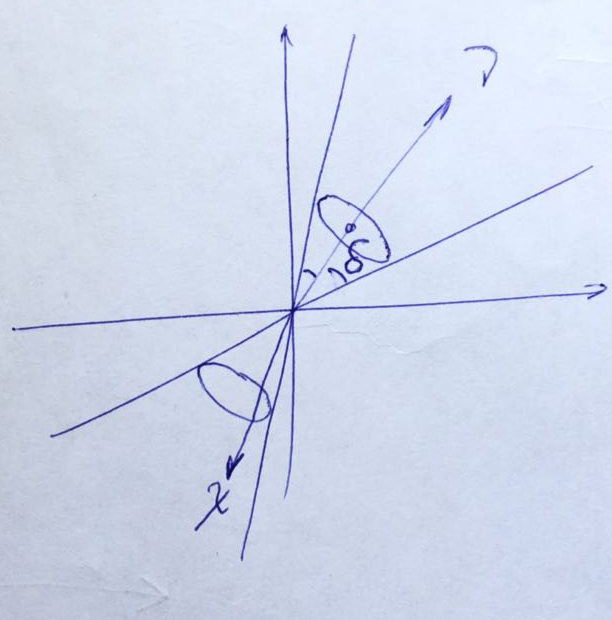
\includegraphics[width=0.48\linewidth]{figs/cone_by_hand}
	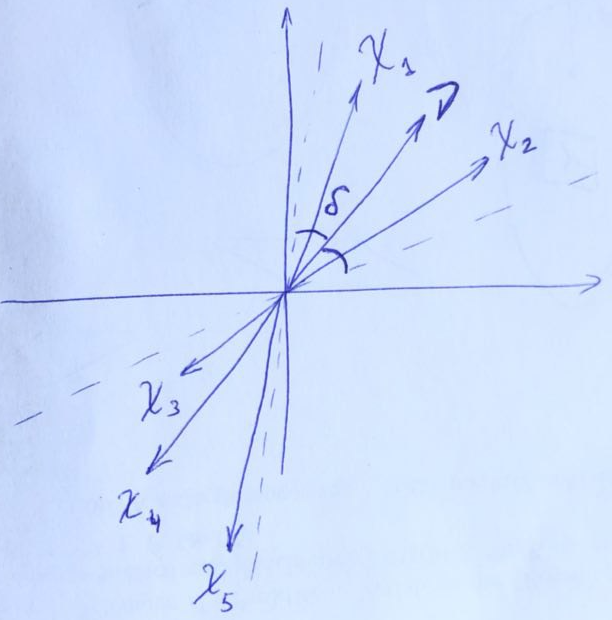
\includegraphics[width=0.48\linewidth]{figs/multicorr_by_hand} 
	\caption{$\textsf{Cone}_{\delta}(\bnu)$ + $\delta$-multicorrelation}
\end{figure}

There is a link between QPFS matrices $\bQ_x$, $\bQ_y$ and defined $\delta$-multicorrelation.
If we binarize the matrices and put 1's for the entries which are larger or equal to $\delta$ and 0's -- otherwise, we will get the adjacency matrices of some graphs~$G_{\bX}$ and $G_{\bY}$. The edges in these graphs are pairs of vertices which are $\delta$-correlated. The cliques in these adjacency matrices are the feature and the target subsets which are $\delta$-multicorrelated. All vertices in~$G_{\bX}$ which are connected with the vertice $i$ refer to features that lies in $\textsf{Cone}_{\delta}(\bchi_i)$. Similarly, all vertices in~$G_{\bY}$ which are connected with the vertice $k$ refer to targets that lies in $\textsf{Cone}_{\delta}(\bnu_k)$.

The binarized QPFS matrix~$\bB$ defines a bipartite graph~$G_{\bX\bY}$, where first part corresponds to the features and the second -- to targets. In this notation the features that are non-relevant to targets are given by the vertices from the first part which are not connected to any vertex from the second part. We call features from the set $\textsf{Cone}(\bnu_j)$ are relevant to the target $\bnu_j$.

We define two hypergraphs $H_{\bX}$ and $H_{\bY}$. The hypergraphs are given by the set of vertices and the set of edges. There are~$n$ vertices in~$H_{\bX}$ and~$r$ vertices in~$H_{\bY}$. The vertices respond to features and targets respectively. Each edge is given by a set of vertices that are $\delta$-multicorrelated.  

We propose the way to categorize all given features into five disjoint categories. 
\begin{enumerate}
	\item Non-relevant features. These features do not belong to any of the sets
	\[
		\bchi_i \notin \textsf{Cone}_{\delta}(\bnu_j) \text{ for } j = 1, \dots, n.
	\]
	In the terms of QPFS algorithm for these features the corresponding rows of the matrix $\bB$ contain only elements less than $\delta$.
	\item Non-correlated features, which are relevant to non-correlated targets. 
	\begin{align*}
		&\exists j \in \{1, \dots, n\}: \, \bchi_i \in \textsf{Cone}_{\delta} (\bnu_j), \\
		&\bchi_{i'} \notin \textsf{Cone}_{\mu} (\bchi_i) \text{ for } i' \in \{1, \dots, n\}: i' \neq i,   \\
		&\bnu_{j'} \notin \textsf{Cone}_{\lambda} (\bnu_j) \text{ for } j' \in \{1, \dots, n\}: j' \neq j.
	\end{align*}
	These features are isolated in the graph~$G_{\bX}$. There is an edge in the graph~$G_{\bX\bY}$ from these features to targets that are isolated in~$G_{\bY}$. 

	\item Non-correlated features, which are relevant to correlated targets:
	\begin{align*}
	&\exists j \in \{1, \dots, n\}: \, \bchi_i \in \textsf{Cone}_{\delta} (\bnu_j), \\
	&\bchi_{i'} \notin \textsf{Cone}_{\mu} (\bchi_i) \text{ for } i' \in \{1, \dots, n\}: i' \neq i, \\
	&\exists j' \in \{1, \dots, n\}: j' \neq j: \,\bnu_{j'} \in \textsf{Cone}_{\lambda} (\bnu_j).
	\end{align*}
	These features are isolated in the graph~$G_{\bX}$. There is an edge in the graph~$G_{\bX\bY}$ from these features to targets that are not isolated in~$G_{\bY}$. 
	
	\item Correlated features, which are relevant to non-correlated targets:
	\begin{align*}
	&\exists j \in \{1, \dots, n\}: \, \bchi_i \in \textsf{Cone}_{\delta} (\bnu_j), \\
	&\exists i' \in \{1, \dots, n\}: i' \neq i: \,\bchi_{i'} \in \textsf{Cone}_{\mu} (\bchi_i),  \\
	&\bnu_{j'} \notin \textsf{Cone}_{\lambda} (\bnu_j) \text{ for } j' \in \{1, \dots, n\}: j' \neq j.
	\end{align*}
	These features are not isolated in the graph~$G_{\bX}$. There is an edge in the graph~$G_{\bX\bY}$ from these features to targets that are isolated in~$G_{\bY}$. 

	\item Correlated features, which are relevant to correlated targets:
	\begin{align*}
	&\exists j \in \{1, \dots, n\}: \, \bchi_i \in \textsf{Cone}_{\delta} (\bnu_j), \\
	&\exists i' \in \{1, \dots, n\}: i' \neq i: \,\bchi_{i'} \in \textsf{Cone}_{\mu} (\bchi_i),  \\
	&\exists j' \in \{1, \dots, n\}: j' \neq j: \,\bnu_{j'} \in \textsf{Cone}_{\lambda} (\bnu_j).
	\end{align*}
	These features are not isolated in the graph~$G_{\bX}$. There is an edge in the graph~$G_{\bX\bY}$ from these features to targets that are not isolated in~$G_{\bY}$.
\end{enumerate}

\end{document}
